% frame 2
\begin{frame}
  \frametitle{About the Project}
    \begin{itemize}
      \item Audio processing
      \item Keyboard controlled
      \item VGA-compliant GUI
        \begin{itemize}
          \item Settings
          \item Signal status -- Pre- and Post-processing
        \end{itemize}
    \end{itemize}
\end{frame}

%frame 3
\begin{frame}
  \frametitle{First Layer of Modules}
    \begin{figure}
      \centering
      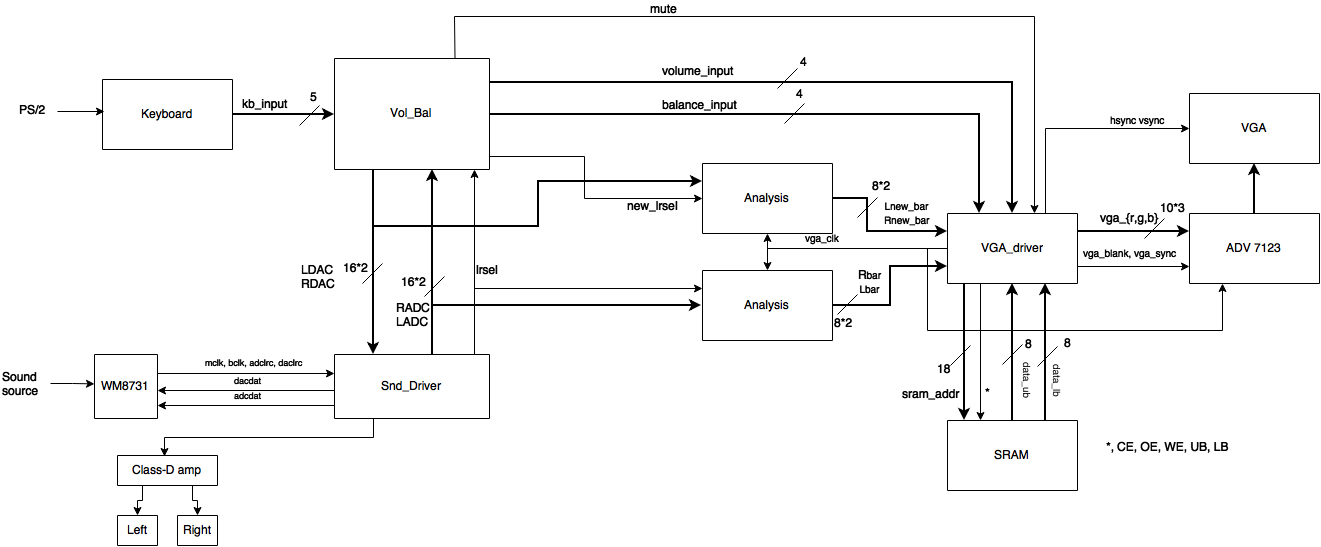
\includegraphics[scale=.23]{overview}
    \end{figure}
\end{frame}

% frame 4
\begin{frame}
  \frametitle{\texttt{Keyboard}}
    \begin{itemize}
      \item PS/2 keyboard, \emph{one hot encoded}
      \item Volume and Balance adjustment, Mute
      \item Scan codes passed into a '1'-set shift register
        \begin{itemize}
          \item Once the startbit is shifted out, the 3:rd byte is checked
          \item Compare with expected values
        \end{itemize}
    \end{itemize}
    \begin{figure}
      \centering
      \begin{tabular}{|c|c|c|c|c|}
        \hline
        KEY & MAKE & BREAK & \texttt{kb\_input} & Function\\ \hline
        U ARROW & E0,75 & E0,F0,75 & 00001 & Volume Increase\\ \hline
        L ARROW & E0,6B & E0,F0,6B & 00010 & Balance Bias Left\\ \hline
        D ARROW & E0,72 & E0,F0,72 & 00100 & Volume Decrease\\ \hline
        R ARROW & E0,74 & E0,F0,74 & 01000 & Balance Bias Right\\ \hline
        END		& E0,69 & E0,F0,69 & 10000 & Mute Volume\\ \hline
      \end{tabular}
    \end{figure}
\end{frame}

% frame 5
\begin{frame}
  \frametitle{\texttt{Snd\_Driver}}
    \begin{itemize}
      \item Identical function as the one in \emph{Lab 4}\\ (\texttt{Vol\_Bal} replaces \texttt{Application})
        \begin{figure}
          \centering
          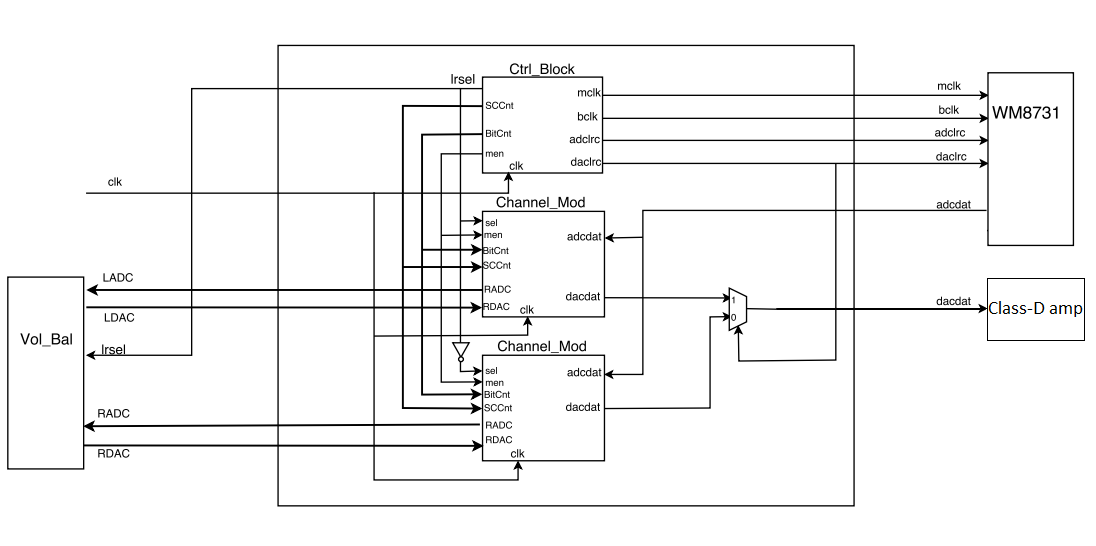
\includegraphics[scale=.37]{snddriver}
        \end{figure}
    \end{itemize}
\end{frame}

% frame 6a
\begin{frame}
  \frametitle{\texttt{Vol\_Bal} (1)}
    \begin{itemize}
      \item Sub-module \texttt{Current\_Vol\_Bal} holds current values for volume, balance and mute
      \item Sub-module \texttt{Adjustment} $$A_{new} = A_{old} \cdot (1/\sqrt{2})^{n}$$
    \end{itemize}
    \begin{figure}
      \centering
      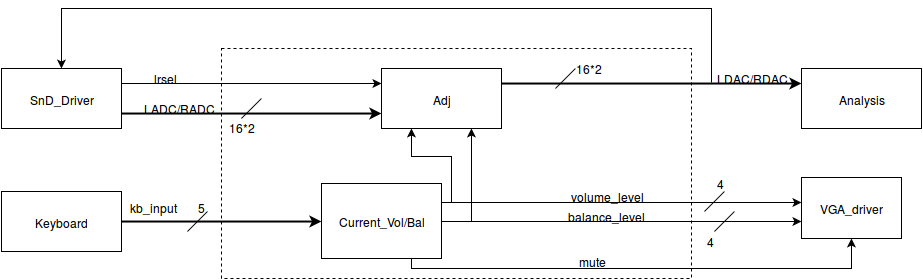
\includegraphics[scale=.33]{volbal}
    \end{figure}
\end{frame}


% frame 6b
\begin{frame}
  \frametitle{\texttt{Vol\_Bal} (2)}
    \begin{itemize}
      \item Decremental adjustment of the output (volume: 0 to (-30) dB, balance: 5 linear steps of bias per channel)
      \item ``Mute'' blanks $A_{new}$ values to \texttt{\{L/R\}DAC}
    \end{itemize}
    \begin{figure}
      \centering
      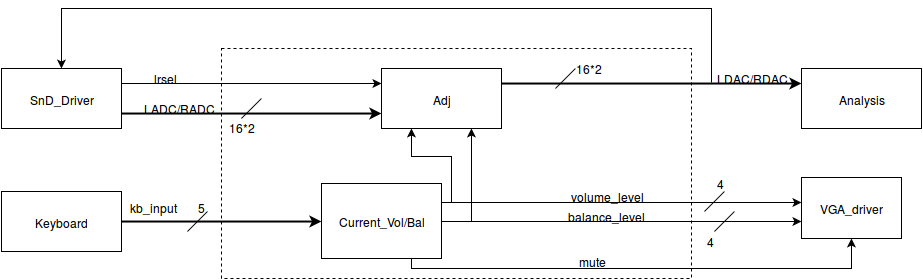
\includegraphics[scale=.33]{volbal}
    \end{figure}
\end{frame}


% frame 7
\begin{frame}
  \frametitle{\texttt{Analysis}}
    \begin{itemize}
      \item Low pass filtering
      \item Forward control signals to \texttt{VGA\_driver}
    \end{itemize}
    \begin{figure}
      \centering
      \begin{tabular}{|l|c|l|}
        \hline
        Name & Type & Description \\    \hline
        \texttt{lrsel} & input & Channel select \\    \hline
        \texttt{\{L,R\}ADC} & input & Left/Right audio input channel \\    \hline
        \texttt{\{L,R\}DAC} & input & Left/Right audio output channel \\    \hline
        \texttt{\{L,R\}new\_bar} & output & Bar amplitude, post-processing\\    \hline
        \texttt{\{L,R\}bar} & output & Bar amplitude, pre-processing\\    \hline
      \end{tabular}
    \end{figure}
\end{frame}

\begin{frame}
  \frametitle{\texttt{Analysis}}
	\begin{figure}
	  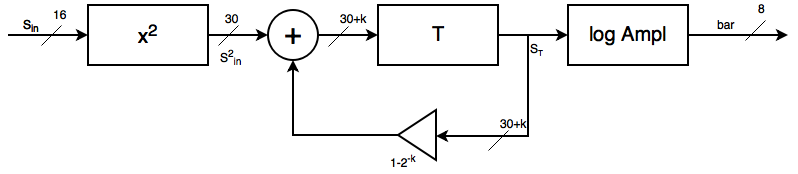
\includegraphics[scale=.35]{lowpass.png}
	  \begin{itemize}
	    \item 100 ms saturation time, $k$ is worked out accordingly
	  \end{itemize}
	  $$\frac{1}{10}\mathrm{\ s} = 2^k\cdot\frac{1}{48800}\Rightarrow 2^k=4880\approx 2^{12}\Rightarrow k = 12$$
	\end{figure}
\end{frame}

% frame 8
\begin{frame}[plain]
  \frametitle{\texttt{VGA-driver}}
    \begin{itemize}
      \item Similar to \emph{Lab 3} 
      \item New sub-modules: \texttt{Bar\_\{Tender,Mixer\}}
    \end{itemize}
    \begin{figure}
      \centering
      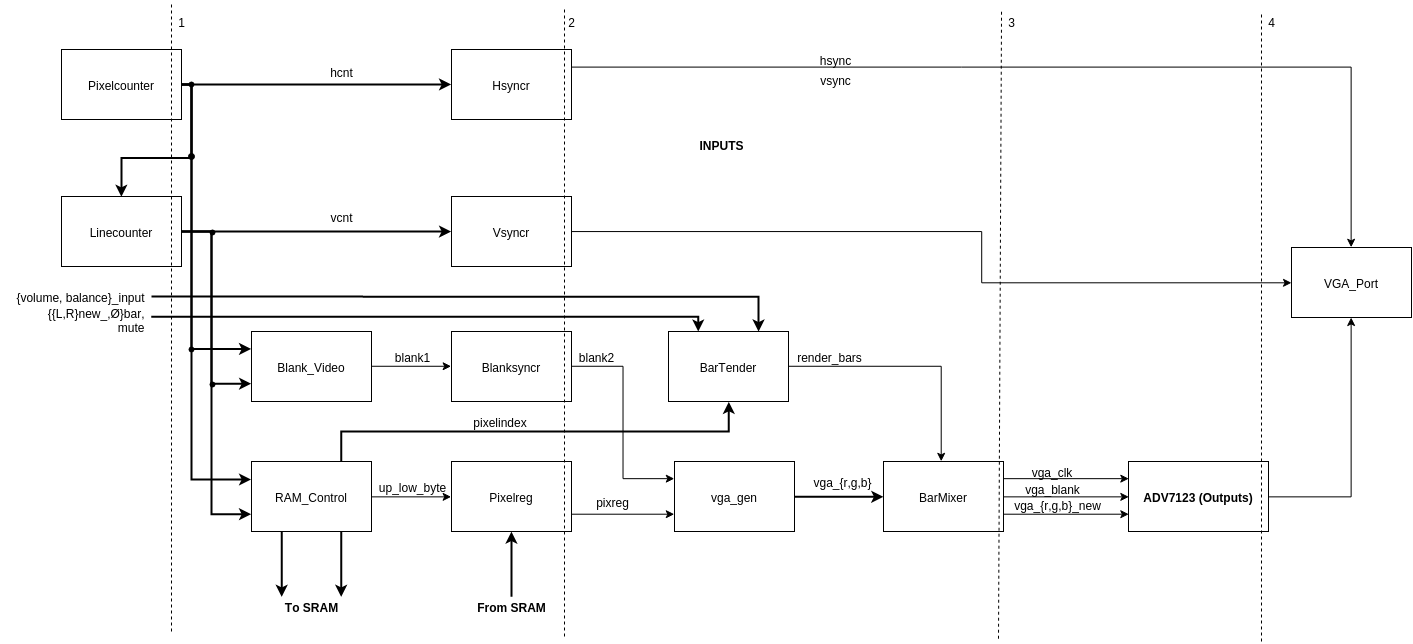
\includegraphics[scale=.23]{vgadrive}
    \end{figure}
\end{frame}

\begin{frame}
  \frametitle{\texttt{VGA-driver}}
    \begin{figure}
      \centering
      \small{
        \begin{tabular}{|l|c|p{6.2cm}|}
          \hline
          Name & Type & Description \\
          \hline
          \texttt{volume\_input} & Input & A 4-bit input containing vol. info.\\
          \hline
          \texttt{balance\_input} & Input & A 4-bit input containing bal. info.\\
          \hline
          \texttt{\{L,R\}bar} & Input & An 8-bit input containing input signal level\\
          \hline
          \texttt{\{L,R\}new\_bar} & Input & An 8-bit input containing manipulated input signal level\\
          \hline
          \texttt{vsync} & Output & Control signal for reading the analysis registers\\
          \hline
        \end{tabular}
      }
    \end{figure}
\end{frame}

% frame 9
\begin{frame}
  \frametitle{\texttt{Bar\_Tender}}
    \begin{figure}
      \centering
      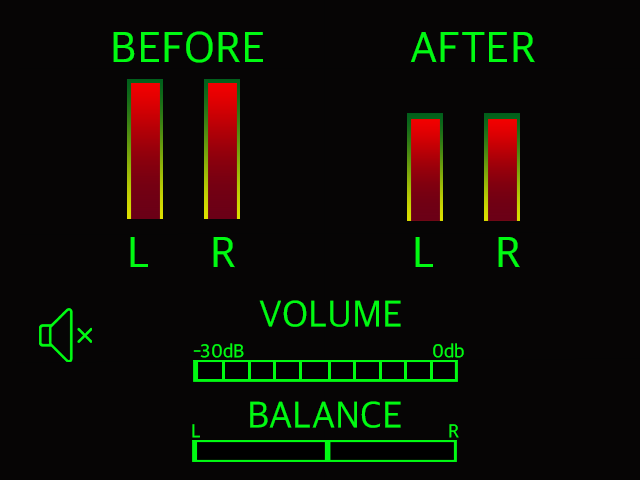
\includegraphics[scale=.25]{UI}
    \end{figure}
    \begin{itemize}
      \item Creates rendering control signal \texttt{render\_bars} for bar graphs (volume, balance, signal strength pre- and post-processing)
      \item Background pre-filled bars are blanked out downwards
    \end{itemize}

\end{frame}

% frame 10
\begin{frame}
  \frametitle{\texttt{Bar\_Mixer}}
    \begin{itemize}
      \item Acts as a multiplexer blanking/enabling bar fill through the control signal \texttt{render\_bars}.
    \end{itemize}
    \begin{figure}
      \centering
      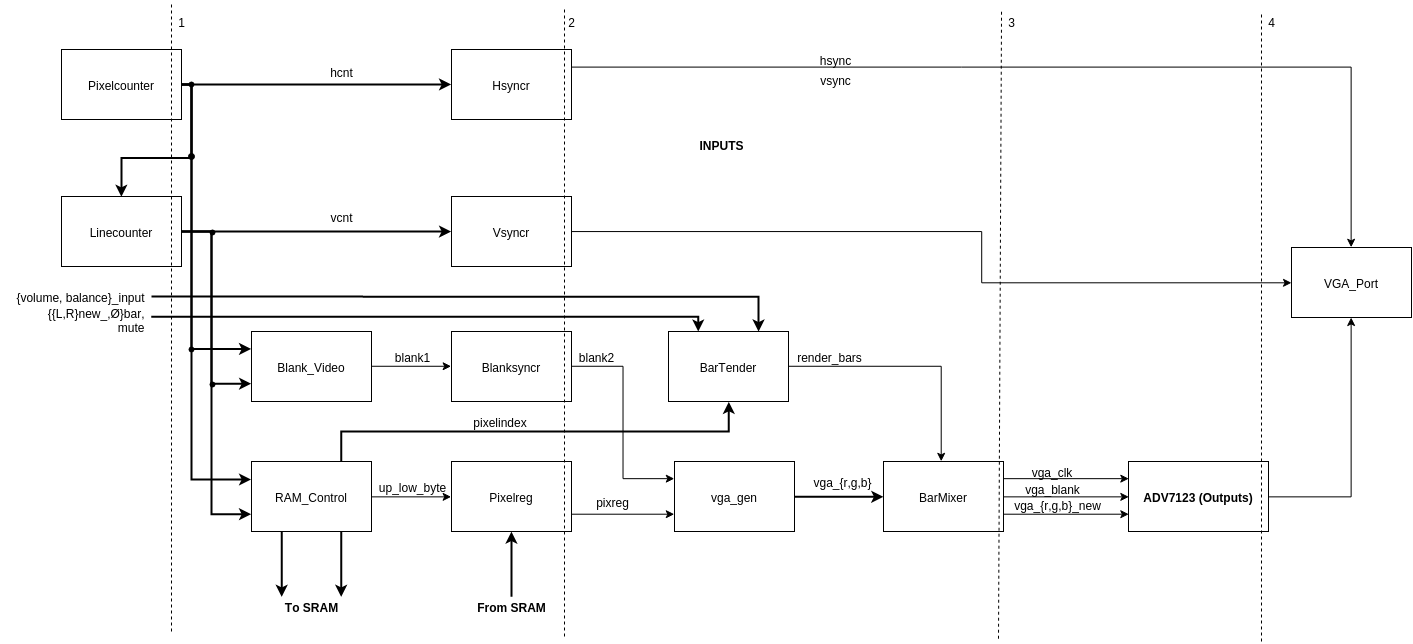
\includegraphics[scale=.23]{vgadrive}
    \end{figure}
\end{frame}
